\section{Electromagnetically Induced Transparency}
Electromagnetically Induced Tranparency is a well known phenomenon in atomic physics but its all-optical analogue has generated a lot of interest in this beautiful natural phenomenon. Basically, EIT is a transparency window in transmission and absorption spectrum. This transparency window is the result of fano interference amoung different transition pathways. There is another similar concept which is known as Autler-Townes Splitting ATS, which also shows a transparency window but it is the result of strong field-driven interactions which causes the energy levels to split.

EIT also enables us to hold control over the optical response of the medium. Basically, EIT is the result of having a strong connection between the light and the matter. Amplitudes of different pathways interfere due to quantum interference effects. These can be used in applications such as all-optical switching, slow light, optical sensing, light storage and quantum information processing.

In photonics, EIT is said to be observed in plasmonic structures, photonic crystals, whispering gallery mode micro cavities and coupled ring micro resonators. These devices can be summed up under one name, photonic devices and by seeing such effects we can say that we can get control of how information and energy travel through our device.

\subsection{EIT in Atoms}
For EIT to happen classically, one may assume that all the oscillating atoms in the medium have came to a hault just to neutralize the incoming field effect and thus these electrons does not contribute in the dielectric of the material. But atoms are small and must be treated quantum mechanically, in which we deal with probability amplitudes and expected value of electron's position. 
\subsection{Three level Atoms}
In a three level system, what really happens quantum mechanically, without disrupting the escence of classical phenomenons, The probability amplitudes of level $\ket{3}$ is driven by two terms in the system. One is being the probability amplitude of the ground state $\ket{1}$ and the other is the oppositely phased and is the probability amplitude of the state $\ket{2}$. These both driving forces are opposite in signs but equal in magnitudes and have a frequecy $\omega_{p}$ and are so balanced that probabilty amplitude of state $\ket{3}$ and the expected value of the amplitude of the sinosoidal motion at every frequency that has been applied is zero. 
One may ask how that opposite phase for transition from the coherent states $\ket{1} \to \ket{2}$ along with the applied field $\omega_{c}$, makes absolute cancellation? Because, we use the laser pulses that generates fast enough laser photons that the phase of transitions is maintain and is the correct phase for cancellation. 

\begin{figure}[h]
\centering
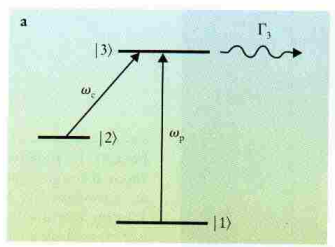
\includegraphics[scale=0.5]{EIT_3levl_atom.png}
\caption{A three-level system where level 3 decays with $\Gamma_{3}$ to states outside the system. [1]}
\end{figure}


\section{Coupled Resonator Induced Transparency (CRIT)}
We can observe EIT in coupled resonator systems as well as in other optical systems like whispering gallery resonators but the scope of this thesis is limited to ring resonators systems only. This kind of geometry (That we discussed in section 2.4) has been promising since a long time in the field of photonics. EIT can be observed in this system by mostly the explaination of classical wave travel and quantum fluctuations. The traveling photon is coupled inside the first ring through evanescent wave and travels inside the ring and acquires a phase shift equal to the round trip inside the optical cavity. When the light source and the phase shifted intracavity field matches so as that the constructive interference is amplified i-e their phases matches perfectly, then at those frequency there is a transparency window in the absorption spectrum i-e a narrow dip, or we see a sharp peak in the transmission spectrum. [2] 

\subsubsection{Transmittance}
Figure 3.2 displays the plot of transmitted intensity vs frequency detuning in a coupled resonator system as shown in fig. 2.16. The parameters used here are couplings $r_{1} = 0.9$ and $r_{2} = 0.999$ and attenuations $a_{1} = 0.88$ and $a_{2} = 0.9999$ for ring 1 and 2 respectively. [2]

\begin{figure}[h]
\centering
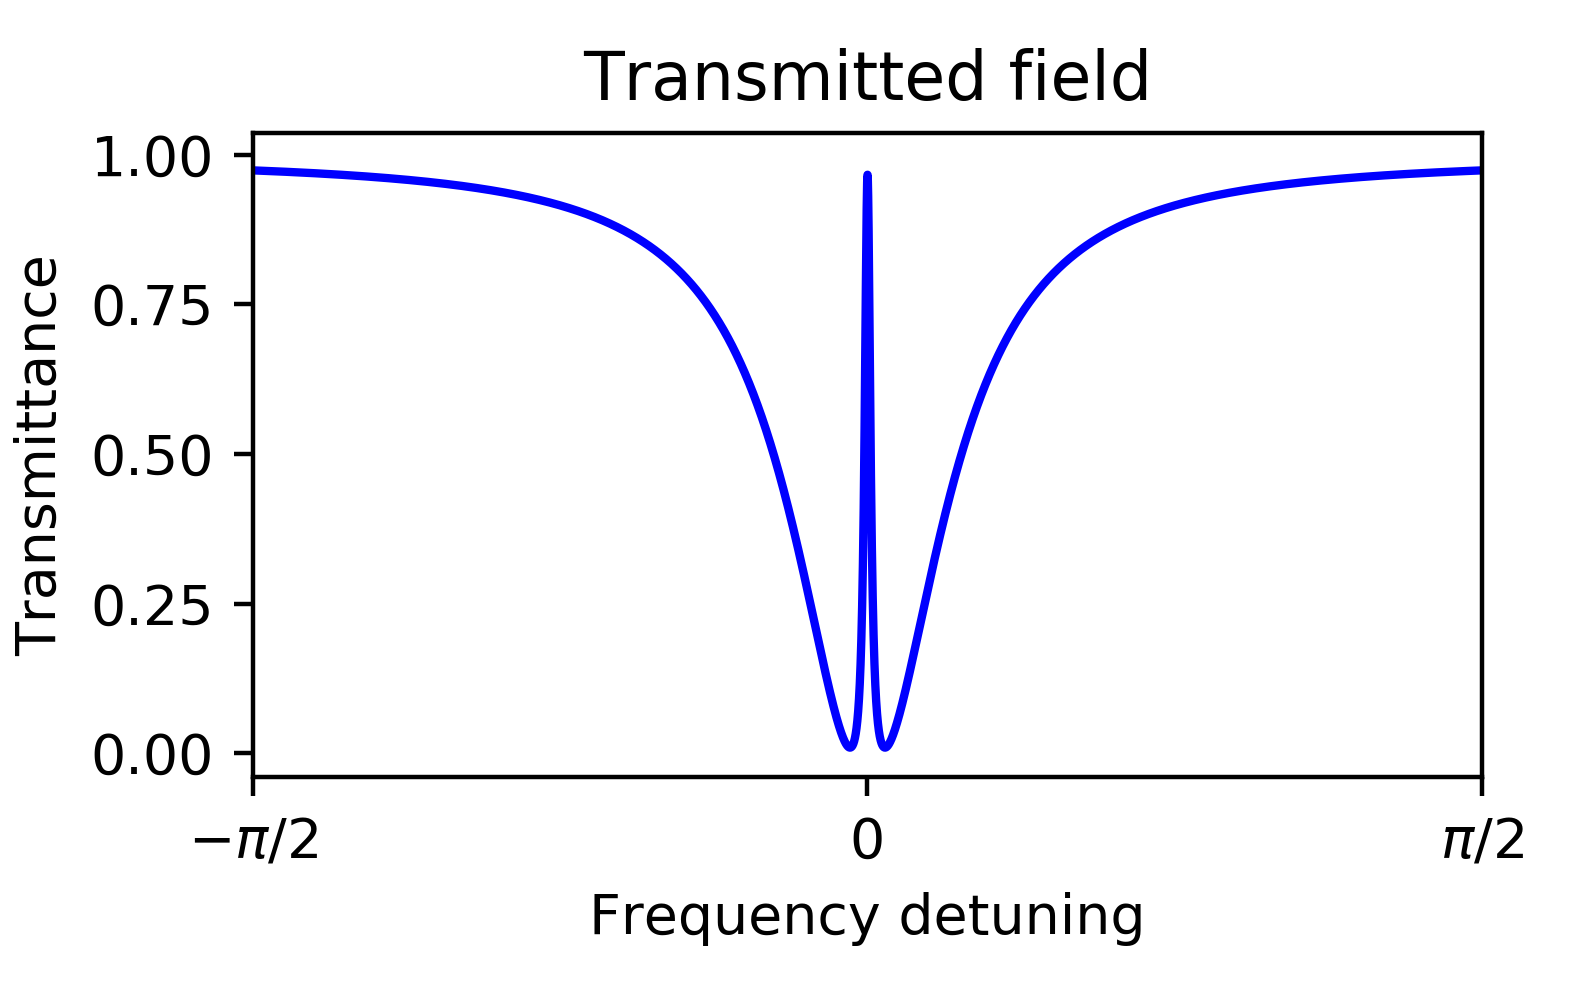
\includegraphics[scale=1]{coupled_ring_EIT1.png}
\caption{EIT observed in a 2 ring resonator system.}
\end{figure}

\subsubsection{Phase}

Now let us look at the phase response of such coupled resonator system. Figure 3.3 shows effective phase of the system in red and Figure 3.4 shows the coupling phase which is the phase between the two coupled rings, in yellow. 

\begin{figure}[h]
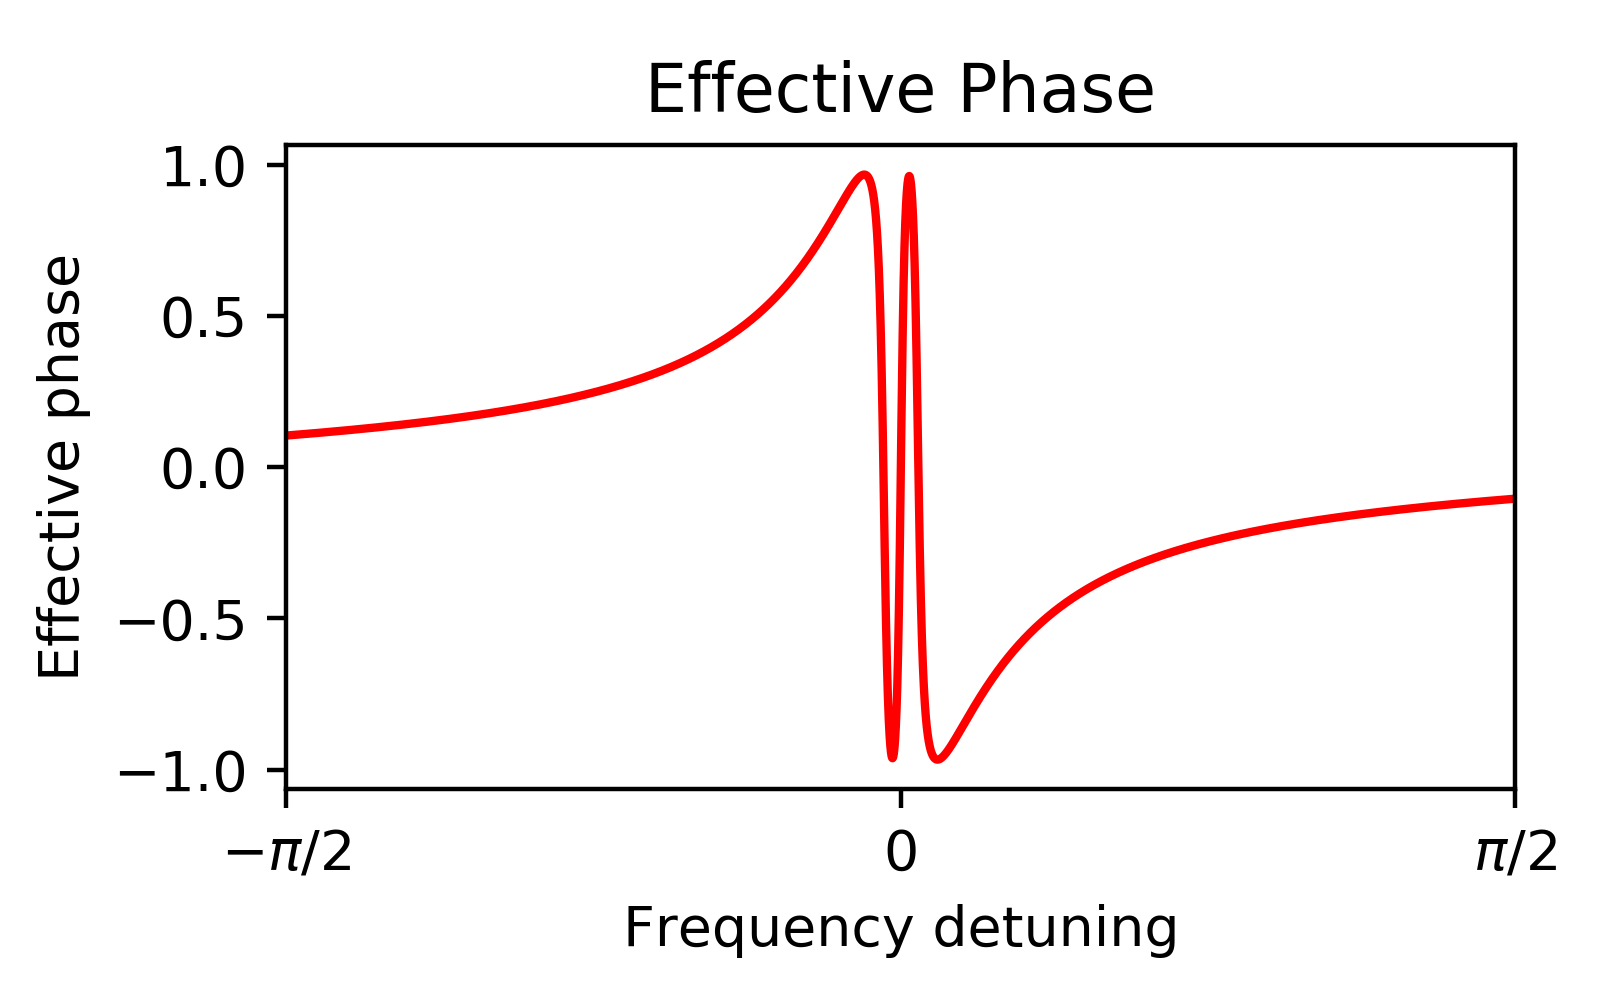
\includegraphics[scale=0.75]{coupled_ring_EIT1_phase.png}
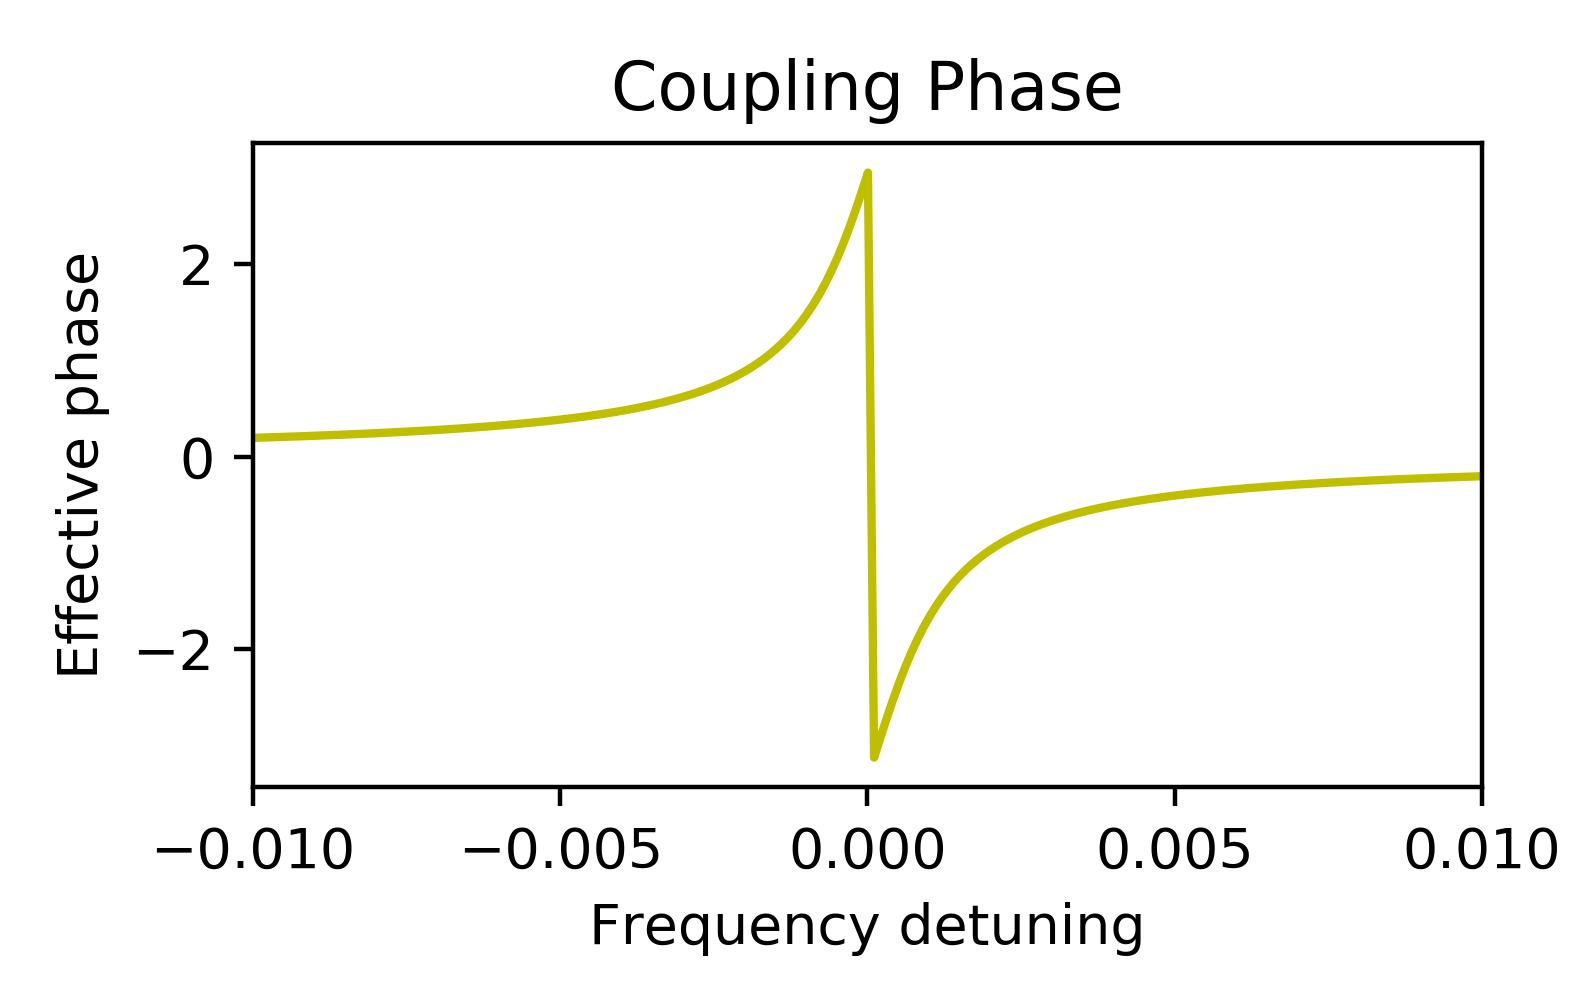
\includegraphics[scale=0.75]{coupled_ring_EIT1_coupling.png}
\caption{Effective phase of the system in red and coupling phase shown in yellow vs frequency detuning.}
\end{figure}

\subsubsection{Effective Phase derivative}
Figure 3.4 shows the derivative of the phase of the system which gives us great information about the group index and group velocity of the system. 
\begin{figure}[h]
\centering
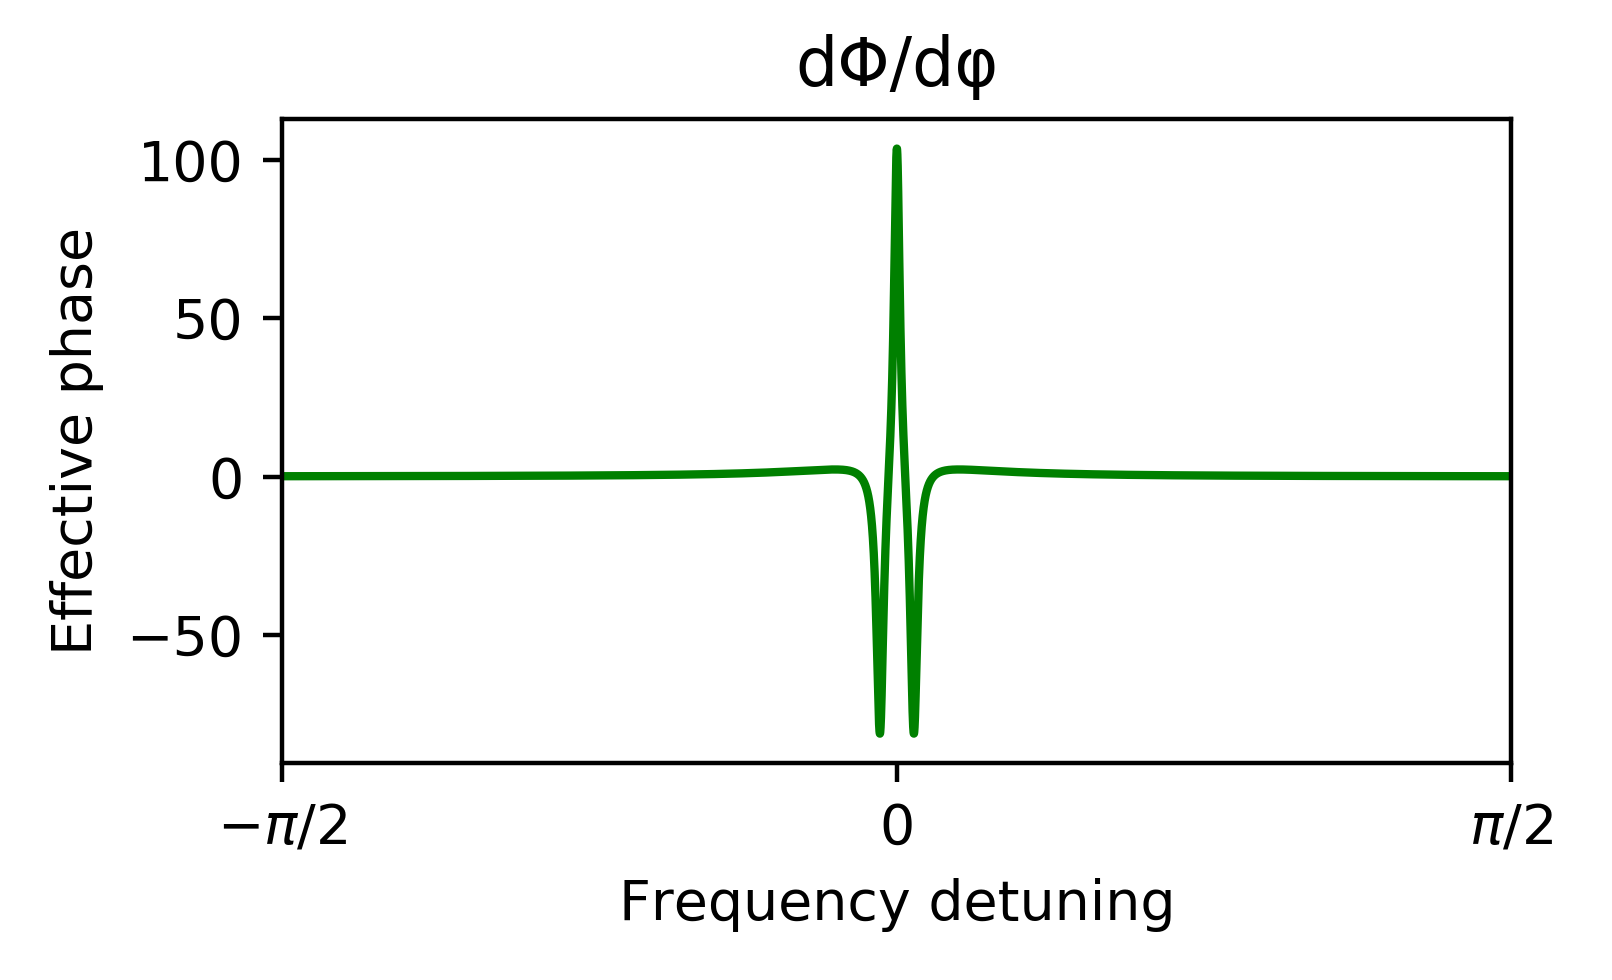
\includegraphics[scale=1]{coupled_ring_EIT1_deri.png}
\caption{Derivative of the phase of the system vs frequency detuning.}
\end{figure}


\subsection{CRIT with gain}
As before, now we are going to observe what changes does the system has when we introduce gain in it. This can be introduced by pumping some monochromatic light source or a laser, in either one of the rings which will drastically incompensate the losses inside the resonator and will increase the overall output transmission of the system even above the incident light source. 
\subsubsection*{Results}
To perform more advanced calculations, it is important to have some understanding of how mpmath works internally and what the possible sources of error are. This section gives an overview of arbitrary-precision binary floating-point arithmetic and some concepts from numerical analysis.Most of the time, using mpmath is simply a matter of setting the desired precision and entering a formula. For verification purposes, a quite (but not always!) reliable technique is to calculate the same thing a second time at a higher precision and verifying that the results agree.

To perform more advanced calculations, it is important to have some understanding of how mpmath works internally and what the possible sources of error are. This section gives an overview of arbitrary-precision binary floating-point arithmetic and some concepts from numerical analysis.


\section{EIA concepts}
To perform more advanced calculations, it is important to have some understanding of how mpmath works internally and what the possible sources of error are. This section gives an overview of arbitrary-precision binary floating-point arithmetic and some concepts from numerical analysis.To perform more advanced calculations, it is important to have some
\subsection{EIA in atoms}
 understanding of how mpmath works internally and what the possible sources of error are. This section gives an overview of arbitrary-precision binary floating-point arithmetic and some concepts from numerical analysis.To perform more advanced calculations, it is important to have some understanding of how mpmath works internally and what the possible sources of error are. 
\subsection{EIA Quantum phenomena} 
 This section gives an overview of arbitrary-precision binary floating-point arithmetic and some concepts from numerical analysis.To perform more advanced calculations, it is important to have some understanding of how mpmath works internally and what the possible sources of error are. This section gives an overview of arbitrary-precision binary floating-point arithmetic and some concepts from numerical analysis.To perform more advanced calculations, it is important to have some understanding of how mpmath works internally and what the possible sources of error are. This section gives an overview of arbitrary-precision binary floating-point arithmetic and some concepts from numerical analysis.To perform more advanced calculations, it is important to have some understanding of how mpmath works internally and what the possible sources of error are.
\section{EIA in resonators} 
 
  This section gives an overview of arbitrary-precision binary floating-point arithmetic and some concepts from numerical analysis.To perform more advanced calculations, it is important to have some understanding of how mpmath works internally and what the possible sources of error are. This section gives an overview of arbitrary-precision binary floating-point arithmetic and some concepts from numerical analysis.
  
\subsection{Coupled resontors induced Absorption}

To perform more advanced calculations, it is important to have some understanding of how mpmath works internally and what the possible sources of error are. This section gives an overview of arbitrary-precision binary floating-point arithmetic and some concepts from numerical analysis.To perform more advanced calculations, it is important to have some understanding of how mpmath works internally and what the possible sources of error are. This section gives an overview of arbitrary-precision binary floating-point arithmetic and some concepts from numerical analysis.
\section{CRIA with gain}
To perform more advanced calculations, it is important to have some understanding of how mpmath works internally and what the possible sources of error are. This section gives an overview of arbitrary-precision binary floating-point arithmetic and some concepts from numerical analysis.To perform more advanced calculations, it is important to have some understanding of how mpmath works internally and what the possible sources of error are. This section gives an overview of arbitrary-precision binary floating-point arithmetic and some concepts from numerical analysis.


\newpage
\section*{References}
\addcontentsline{toc}{section}{References}

\paragraph{\normalfont \large $[1]$ Electromagnetically Induced Transparency, Stephen E. Harris, Physics Today, July 1997 \\ 
\\$[2]$ Coupled-resonator-induced transparency, PHYSICAL REVIEW A 69, 063804 (2004)
\\$[3]$ What is and what is not electromagnetically induced transparency in whispering-gallery microcavities, DOI:10.1038/ncomms6082, Published 24 Oct 2014 \\
\\$[4]$  Induced transparency and absorption in coupled whispering gallery microresonators, PHYSICAL REVIEW A 71, 043804, published 5 April 2005\\
\\$[5]$  }